% -*- TeX-master: "../fat_manual.tex" -*-

\section{RHUL VNA Rohde and Schwartz}
\begin{itemize}
\item \quote{Sweep} \ira \quote{sweepTIme}: continuous = sweep, CW = single freq
\item \texttt{Scale} \ira autoscale
\item \texttt{Span} \ira Center 10GHz, span 16 GHz;
\item \quote{Power BW AVG} to set power, bandwidth;
\item RF ON.
\item \red{When first  connected via ethernet, run  the \quote{rsvna-lv\_2\_42\_0} installer and run  the \quote{Set OPC
      timeout.vi} with 300000ms  = 300 seconds or  larger in the program,  so that the wait  time from the VNA  to PC is
    increased.}
\end{itemize}

\paragraph{VNA} compares the \textbf{phase} and \textbf{amplitude} of an outgoing signal to the one fed into the system.

 \begin{figure}[h]
   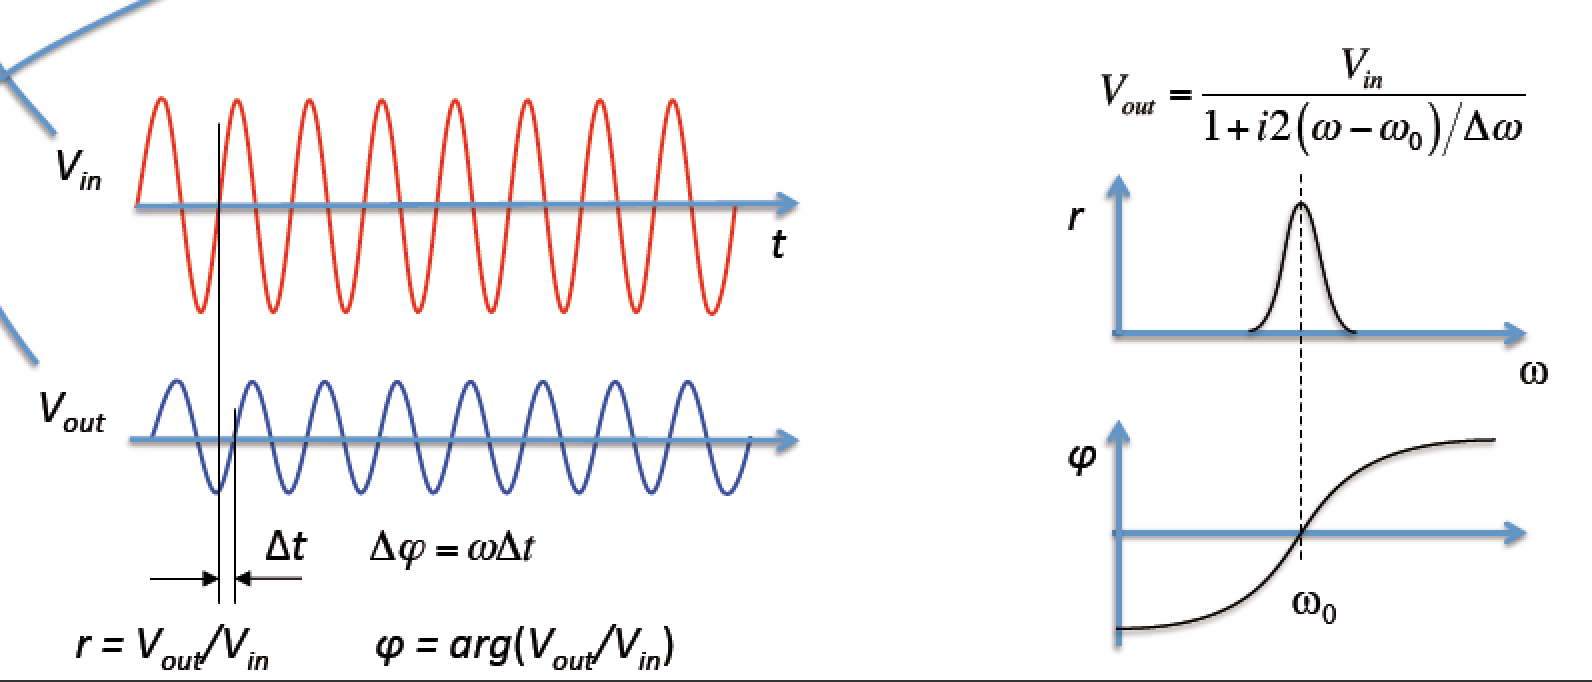
\includegraphics[height=4cm]{vna}
 \end{figure}

 \section{Trigger}
 \label{sec:trigger}

 For two tone measurement set \red{Trigger from sync}

 For Rabi set \red{Free run}

 \subsection{Correct phase}
 \label{sec:correct-phase}

 If the phase is choppy, then do \cmd{click \quote{Offset-embed} \ira \quote{Auto-length}}.

 \subsection{Measure Q factor}
 \label{sec:measure-q-factor}

 To measure q factor of resonator:
 \begin{enumerate}
 \item \cmd{Click \quote{Marker} and select 4 markers};
 \item \cmd{Click \quote{Band filter} \ira \quote{Bandpass reference to max}.} \red{make sure it's set to 3dB};
 \item Markers will  be moved to positions  where the peak falls  off by 3dB (equivalent  to halving) to work  our the Q
   factor
 \end{enumerate}
 \newpage
